% GNUPLOT: LaTeX picture with Postscript
\begingroup
  \makeatletter
  \providecommand\color[2][]{%
    \GenericError{(gnuplot) \space\space\space\@spaces}{%
      Package color not loaded in conjunction with
      terminal option `colourtext'%
    }{See the gnuplot documentation for explanation.%
    }{Either use 'blacktext' in gnuplot or load the package
      color.sty in LaTeX.}%
    \renewcommand\color[2][]{}%
  }%
  \providecommand\includegraphics[2][]{%
    \GenericError{(gnuplot) \space\space\space\@spaces}{%
      Package graphicx or graphics not loaded%
    }{See the gnuplot documentation for explanation.%
    }{The gnuplot epslatex terminal needs graphicx.sty or graphics.sty.}%
    \renewcommand\includegraphics[2][]{}%
  }%
  \providecommand\rotatebox[2]{#2}%
  \@ifundefined{ifGPcolor}{%
    \newif\ifGPcolor
    \GPcolortrue
  }{}%
  \@ifundefined{ifGPblacktext}{%
    \newif\ifGPblacktext
    \GPblacktextfalse
  }{}%
  % define a \g@addto@macro without @ in the name:
  \let\gplgaddtomacro\g@addto@macro
  % define empty templates for all commands taking text:
  \gdef\gplbacktext{}%
  \gdef\gplfronttext{}%
  \makeatother
  \ifGPblacktext
    % no textcolor at all
    \def\colorrgb#1{}%
    \def\colorgray#1{}%
  \else
    % gray or color?
    \ifGPcolor
      \def\colorrgb#1{\color[rgb]{#1}}%
      \def\colorgray#1{\color[gray]{#1}}%
      \expandafter\def\csname LTw\endcsname{\color{white}}%
      \expandafter\def\csname LTb\endcsname{\color{black}}%
      \expandafter\def\csname LTa\endcsname{\color{black}}%
      \expandafter\def\csname LT0\endcsname{\color[rgb]{1,0,0}}%
      \expandafter\def\csname LT1\endcsname{\color[rgb]{0,1,0}}%
      \expandafter\def\csname LT2\endcsname{\color[rgb]{0,0,1}}%
      \expandafter\def\csname LT3\endcsname{\color[rgb]{1,0,1}}%
      \expandafter\def\csname LT4\endcsname{\color[rgb]{0,1,1}}%
      \expandafter\def\csname LT5\endcsname{\color[rgb]{1,1,0}}%
      \expandafter\def\csname LT6\endcsname{\color[rgb]{0,0,0}}%
      \expandafter\def\csname LT7\endcsname{\color[rgb]{1,0.3,0}}%
      \expandafter\def\csname LT8\endcsname{\color[rgb]{0.5,0.5,0.5}}%
    \else
      % gray
      \def\colorrgb#1{\color{black}}%
      \def\colorgray#1{\color[gray]{#1}}%
      \expandafter\def\csname LTw\endcsname{\color{white}}%
      \expandafter\def\csname LTb\endcsname{\color{black}}%
      \expandafter\def\csname LTa\endcsname{\color{black}}%
      \expandafter\def\csname LT0\endcsname{\color{black}}%
      \expandafter\def\csname LT1\endcsname{\color{black}}%
      \expandafter\def\csname LT2\endcsname{\color{black}}%
      \expandafter\def\csname LT3\endcsname{\color{black}}%
      \expandafter\def\csname LT4\endcsname{\color{black}}%
      \expandafter\def\csname LT5\endcsname{\color{black}}%
      \expandafter\def\csname LT6\endcsname{\color{black}}%
      \expandafter\def\csname LT7\endcsname{\color{black}}%
      \expandafter\def\csname LT8\endcsname{\color{black}}%
    \fi
  \fi
  \setlength{\unitlength}{0.0500bp}%
  \begin{picture}(5668.00,4534.00)%
    \gplgaddtomacro\gplbacktext{%
      \csname LTb\endcsname%
      \put(946,704){\makebox(0,0)[r]{\strut{}-1.5}}%
      \csname LTb\endcsname%
      \put(946,1100){\makebox(0,0)[r]{\strut{}-1}}%
      \csname LTb\endcsname%
      \put(946,1496){\makebox(0,0)[r]{\strut{}-0.5}}%
      \csname LTb\endcsname%
      \put(946,1892){\makebox(0,0)[r]{\strut{} 0}}%
      \csname LTb\endcsname%
      \put(946,2288){\makebox(0,0)[r]{\strut{} 0.5}}%
      \csname LTb\endcsname%
      \put(946,2685){\makebox(0,0)[r]{\strut{} 1}}%
      \csname LTb\endcsname%
      \put(946,3081){\makebox(0,0)[r]{\strut{} 1.5}}%
      \csname LTb\endcsname%
      \put(946,3477){\makebox(0,0)[r]{\strut{} 2}}%
      \csname LTb\endcsname%
      \put(946,3873){\makebox(0,0)[r]{\strut{} 2.5}}%
      \csname LTb\endcsname%
      \put(946,4269){\makebox(0,0)[r]{\strut{} 3}}%
      \csname LTb\endcsname%
      \put(1184,484){\makebox(0,0){\strut{} 250}}%
      \csname LTb\endcsname%
      \put(1825,484){\makebox(0,0){\strut{} 500}}%
      \csname LTb\endcsname%
      \put(2467,484){\makebox(0,0){\strut{} 750}}%
      \csname LTb\endcsname%
      \put(3108,484){\makebox(0,0){\strut{} 1000}}%
      \csname LTb\endcsname%
      \put(3750,484){\makebox(0,0){\strut{} 1250}}%
      \csname LTb\endcsname%
      \put(4391,484){\makebox(0,0){\strut{} 1500}}%
      \colorrgb{1.00,0.00,0.00}%
      \put(4523,704){\makebox(0,0)[l]{\strut{}-40}}%
      \colorrgb{1.00,0.00,0.00}%
      \put(4523,1100){\makebox(0,0)[l]{\strut{}-30}}%
      \colorrgb{1.00,0.00,0.00}%
      \put(4523,1496){\makebox(0,0)[l]{\strut{}-20}}%
      \colorrgb{1.00,0.00,0.00}%
      \put(4523,1892){\makebox(0,0)[l]{\strut{}-10}}%
      \colorrgb{1.00,0.00,0.00}%
      \put(4523,2288){\makebox(0,0)[l]{\strut{} 0}}%
      \colorrgb{1.00,0.00,0.00}%
      \put(4523,2685){\makebox(0,0)[l]{\strut{} 10}}%
      \colorrgb{1.00,0.00,0.00}%
      \put(4523,3081){\makebox(0,0)[l]{\strut{} 20}}%
      \colorrgb{1.00,0.00,0.00}%
      \put(4523,3477){\makebox(0,0)[l]{\strut{} 30}}%
      \colorrgb{1.00,0.00,0.00}%
      \put(4523,3873){\makebox(0,0)[l]{\strut{} 40}}%
      \colorrgb{1.00,0.00,0.00}%
      \put(4523,4269){\makebox(0,0)[l]{\strut{} 50}}%
      \csname LTb\endcsname%
      \put(176,2486){\rotatebox{-270}{\makebox(0,0){\strut{}Diffraction Peak Deviation / $\%$}}}%
      \colorrgb{1.00,0.00,0.00}%
      \put(5160,2486){\rotatebox{270}{\makebox(0,0){\strut{}Debye-Scherrer Width Deviation / $\%$}}}%
      \csname LTb\endcsname%
      \put(2734,154){\makebox(0,0){\strut{}Solvent Osmolality / mOsm kg$^{-1}$}}%
    }%
    \gplgaddtomacro\gplfronttext{%
    }%
    \gplbacktext
    \put(0,0){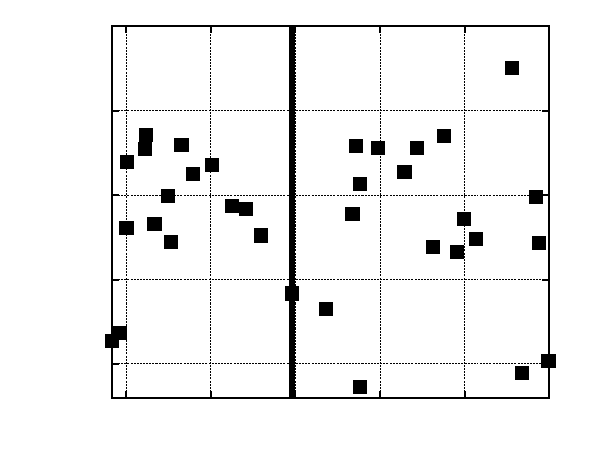
\includegraphics{CaelyxSucroseContinuousWAXSDiffraction}}%
    \gplfronttext
  \end{picture}%
\endgroup
